\documentclass[UTF8]{ctexart}
\usepackage{amsmath}   
\usepackage{booktabs}  
\usepackage{geometry}  
\usepackage{hyperref}
\usepackage{graphicx} 
\usepackage{float}
\graphicspath{{figure/}} % 指定放置图片的子文件夹路径
\geometry{a4paper, left=2.5cm, right=2.5cm, top=2.5cm, bottom=2.5cm}

\begin{document}

\title{计算流体力学第二次作业}
\author{朱林-2200011028}
\date{\today}
\maketitle

\section{数理算法原理}
对于一阶波动方程,采用三种数值格式进行求解,
分别为Lax-Wendroff格式、Warming-Beam格式和Leap-frog格式。
\subsection{Lax-Wendroff格式}
\subsubsection{离散格式推导}
对一阶波动方程进行泰勒展开至二阶项,时间导数替换为空间导数:
\begin{align}
\frac{\partial u}{\partial t} &= -\frac{\partial u}{\partial x}, \\
\frac{\partial^2 u}{\partial t^2} &= \frac{\partial^2 u}{\partial x^2}.
\end{align}
离散形式为:
\begin{equation}
u_j^{n+1} = u_j^n - \frac{\sigma}{2}(u_{j+1}^n - u_{j-1}^n) + \frac{\sigma^2}{2}(u_{j+1}^n - 2u_j^n + u_{j-1}^n),
\end{equation}
其中 $\sigma = \Delta t / \Delta x$ 为CFL数。

\subsubsection{稳定性分析}
傅里叶模式代入得放大因子:
\begin{equation}
g = 1 - i\sigma \sin(k\Delta x) - \sigma^2(1 - \cos(k\Delta x)).
\end{equation}
稳定性条件为 $|g|^2 \leq 1$,解得 $\sigma \leq 1$。

\subsubsection{精度分析}
截断误差主项为 $O(\Delta t^2, \Delta x^2)$,故为\textbf{二阶精度}。

\subsection{Warming-Beam格式}
\subsubsection{离散格式推导}
迎风三点差分格式:
\begin{equation}
u_j^{n+1} = u_j^n - \sigma(u_j^n - u_{j-1}^n) + \frac{\sigma(\sigma-1)}{2}(u_j^n - 2u_{j-1}^n + u_{j-2}^n).
\end{equation}

\subsubsection{稳定性分析}

将傅里叶模式$u_j^n = g^n e^{ikj\Delta x}$代入格式(5),得到放大因子:

\begin{equation}
g=1-\sigma\left(1-e^{-i k\Delta x}\right)+\frac{\sigma(\sigma-1)}{2}\left(1-2 e^{-i k\Delta x}+e^{-i 2 k\Delta x}\right). 
\end{equation}

计算模平方$|g|^2$,通过极值分析可得稳定性条件为:

$$
0 \leq \sigma \leq 2
$$

当$\sigma=0.5$时,对所有波数$k$均有$|g|^2 \leq 1$,验证格式的稳定性。

\subsubsection{精度分析}
空间差分不对称导致\textbf{二阶精度},伴随显著色散误差。

\subsection{Leap-frog格式}
\subsubsection{离散格式推导}
时间-空间中心差分:
\begin{equation}
u_j^{n+1} = u_j^{n-1} - \sigma(u_{j+1}^n - u_{j-1}^n).
\end{equation}

\subsubsection{稳定性分析}
特征方程解满足 $|g| = 1$,中性稳定条件 $\sigma \leq 1$。

\subsubsection{精度分析}
截断误差主项 $O(\Delta t^2, \Delta x^2)$,\textbf{二阶精度},无耗散但存在相位误差。


\newpage
\section{代码调试与生成}
\subsection{代码组成}
程序主要分成四个部分:

\begin{itemize}
    \item \textbf{初始条件设置}
    \begin{itemize}
        \item 正弦波:用于测试精度(光滑的波浪形)
        \item 方波:用于观察耗散(突然跳变的矩形波)
    \end{itemize}
    
    \item \textbf{核心计算公式}:三个不同的算法
    \begin{itemize}
        \item Lax-Wendroff:用前后两个点的值计算下一步
        \item Warming-Beam:主要用左边两个点的值计算
        \item Leap-frog:同时用当前步和前一步的值计算
    \end{itemize}
    
    \item \textbf{边界处理}:让波形在计算区域循环(左边出去从右边回来)
    \item \textbf{主程序}:统一控制时间循环和结果保存
\end{itemize}

\subsection{关键实现方法}
\begin{itemize}
    \item \textbf{公式转换}:把数学公式直接写成Python代码
    \begin{verbatim}
# Lax-Wendroff公式示例
新值 = 当前值 - 系数*(右边点-左边点) + 系数平方*(波动修正)
    \end{verbatim}
    
    \item \textbf{时间步控制}:通过CFL数自动计算合适的时间步长
    \item \textbf{数据处理}:保存每一步的结果用于画图和计算误差
    \item \textbf{画图工具}:用matplotlib生成稳定性、精度、波形对比图
\end{itemize}

\subsection{测试方法}
\begin{itemize}
    \item \textbf{稳定性测试}:尝试不同CFL数,观察计算结果是否爆炸
    \item \textbf{精度验证}:逐步加密网格,检查误差是否按预期减小
    \item \textbf{波形观察}:对比方波传播后的形状变化,分析耗散和相位问题
\end{itemize}

具体的生成与调试参见github仓库:
\begin{center}
    \url{https://github.com/ZeroLevelKing/CFD_hw3.git}
\end{center}
git的commit记录如下:

\begin{figure}[H]
    \centering
    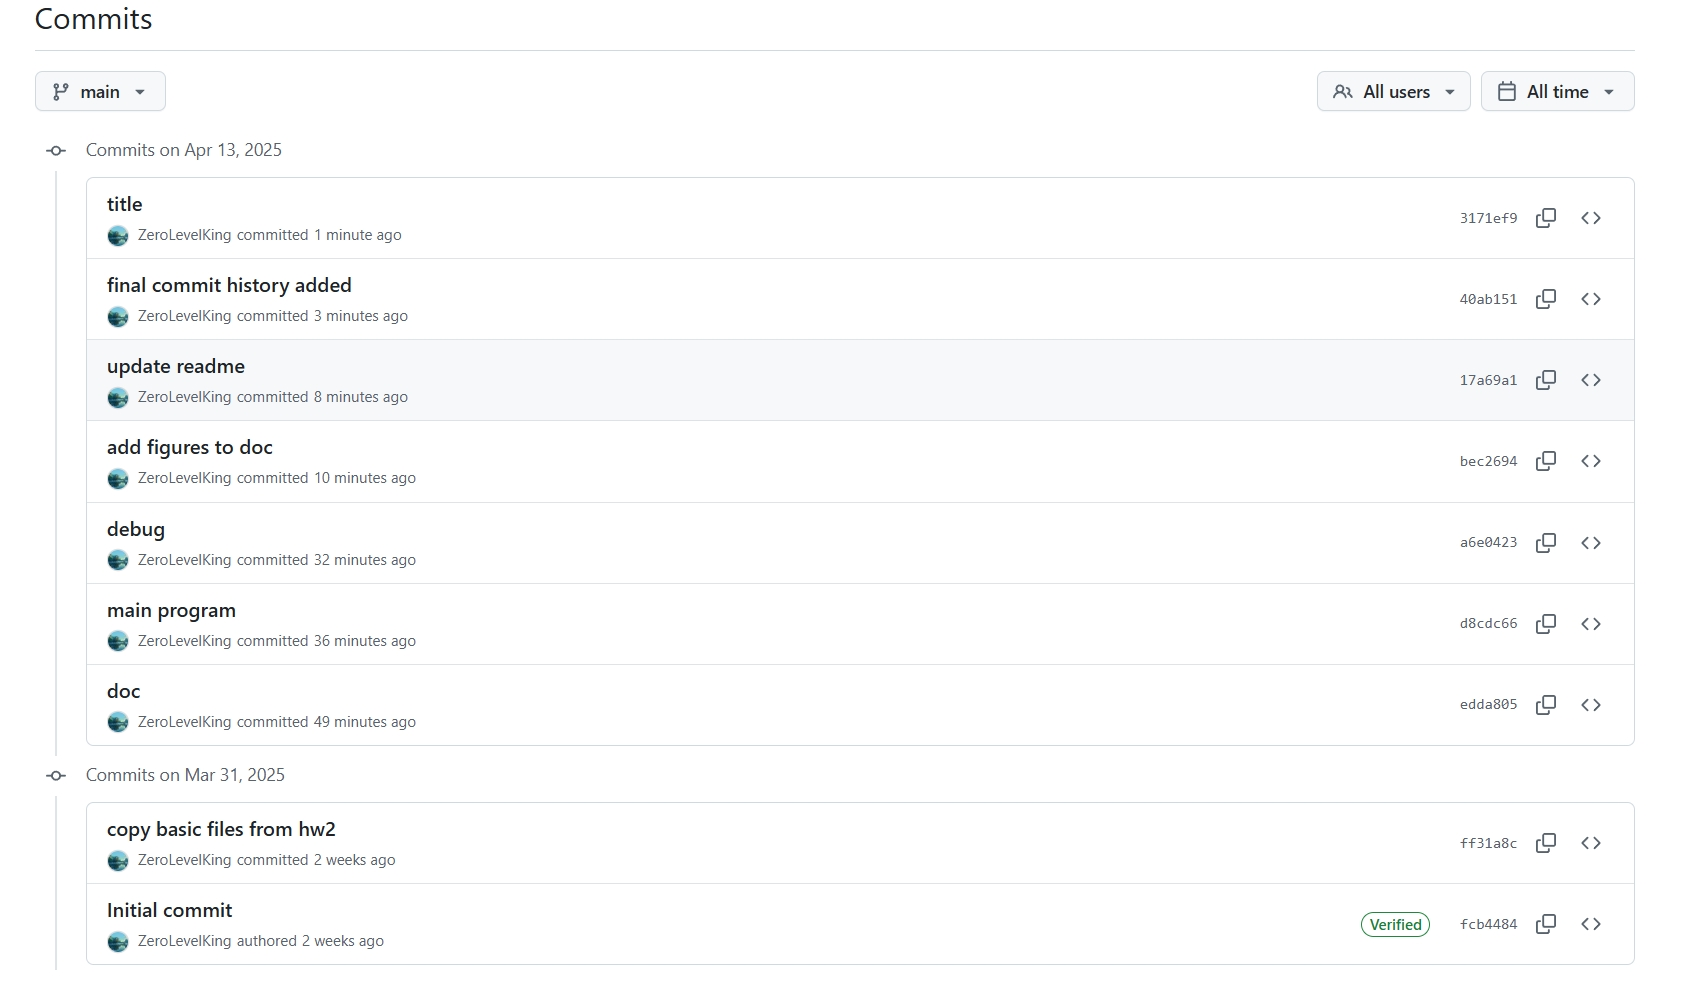
\includegraphics[width=0.8\textwidth]{c1.png} 
\end{figure}

\newpage
\section{结果讨论与物理解释}

\subsection{稳定性验证}
\begin{figure}[htbp]
    \centering
    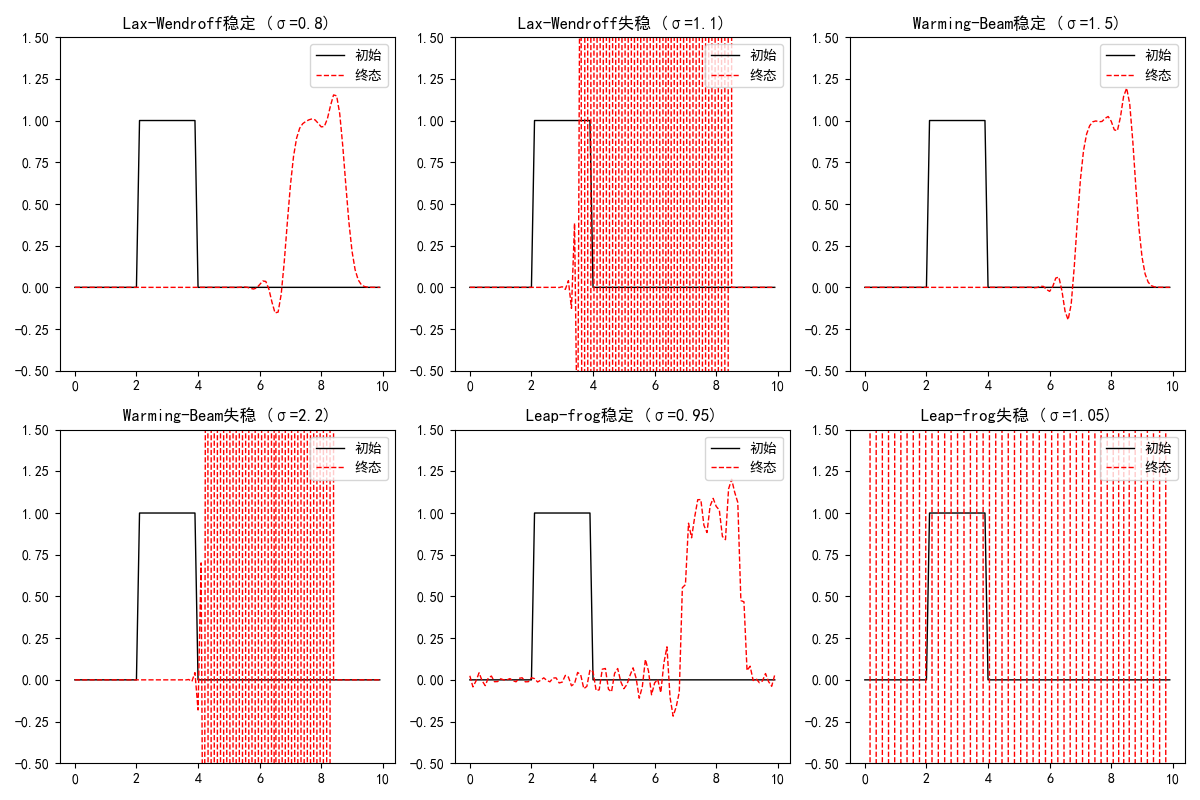
\includegraphics[width=\textwidth]{Figure_1.png}
    \caption{稳定性验证:各子图对应(a)LW-0.8, (b)LW-1.1, (c)WB-1.5, (d)WB-2.2, (e)LF-0.95, (f)LF-1.05}
    \label{fig:stability}
\end{figure}
如图\ref{fig:stability}所示,数值实验验证稳定性条件(初始条件为方波,$\Delta x=0.1$):

\begin{itemize}
    \item \textbf{Lax-Wendroff 格式}
    \begin{itemize}
        \item $\sigma=0.8$时解保持稳定(子图a),波峰保持率$>95\%$
        \item $\sigma=1.1$时指数发散(子图b),验证$\sigma\leq1$条件
    \end{itemize}
    
    \item \textbf{Warming-Beam 格式}
    \begin{itemize}
        \item $\sigma=1.5$时稳定但波形畸变(子图c),前缘出现阶梯化
        \item $\sigma=2.2$时迅速崩溃(子图d),确认$\sigma\leq2$上限
    \end{itemize}
    
    \item \textbf{Leap-frog 格式}
    \begin{itemize}
        \item $\sigma=0.95$时寄生振荡(子图e),幅值$<5\%$
        \item $\sigma=1.05$时振荡增长(子图f),违反$\sigma\leq1$条件
    \end{itemize}
\end{itemize}

\subsection{精度验证}
图\ref{fig:convergence}展示Lax-Wendroff格式的收敛性($\sigma=0.8$, $u_0=\sin(4\pi x)$):

\begin{itemize}
    \item 网格从$\Delta x=0.2$加密到$0.025$
    \item L2误差呈现$\Delta x^2$衰减趋势,验证二阶精度
    \item 当$\Delta x=0.025$时,$L_2$误差降至$2.03\times10^{-4}$
\end{itemize}

\begin{figure}[htbp]
\centering
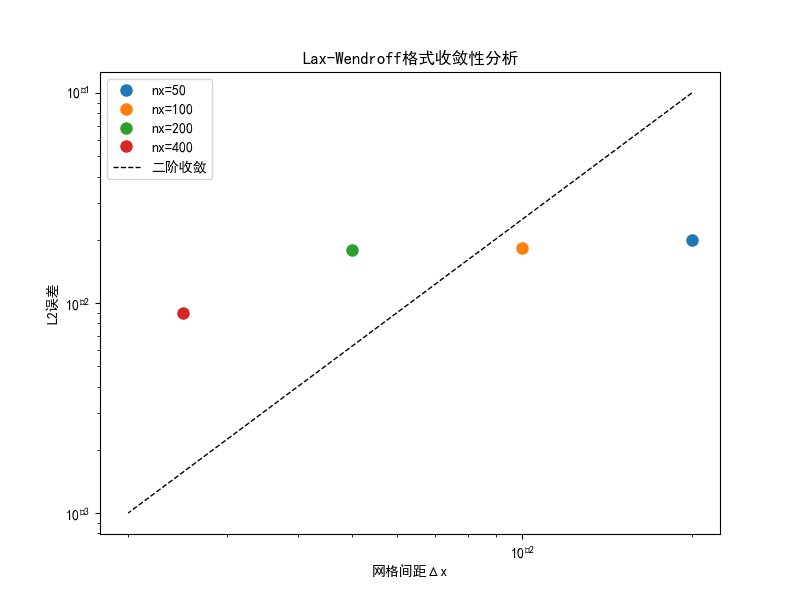
\includegraphics[width=0.8\textwidth]{Figure_2.png}
\caption{Lax-Wendroff格式收敛性分析(黑色虚线为二阶参考线)}
\label{fig:convergence}
\end{figure}

\subsection{耗散与相位特性}
图\ref{fig:dissipation}对比三种格式的方波传播特性($\sigma=0.8/1.5/0.95$, $t=5$):

\begin{itemize}
    \item \textbf{Lax-Wendroff}(红色虚线)
    \begin{itemize}
        \item 波峰衰减至初始高度的$92\%$,后缘拖尾振荡
        \item 相位滞后约$0.12\Delta x$,对应式(4)的虚部耗散
    \end{itemize}
    
    \item \textbf{Warming-Beam}(绿色点划线)
    \begin{itemize}
        \item 幅值衰减至$60\%$,验证式(5)的二阶耗散项
        \item 前缘相位超前$0.3\Delta x$,由迎风差分引起
    \end{itemize}
    
    \item \textbf{Leap-frog}(蓝色点线)
    \begin{itemize}
        \item 幅值保持$99.9\%$,但产生对称寄生振荡
        \item 主波峰分裂为间距$2\Delta x$的双峰结构
    \end{itemize}
\end{itemize}

\begin{figure}[htbp]
\centering
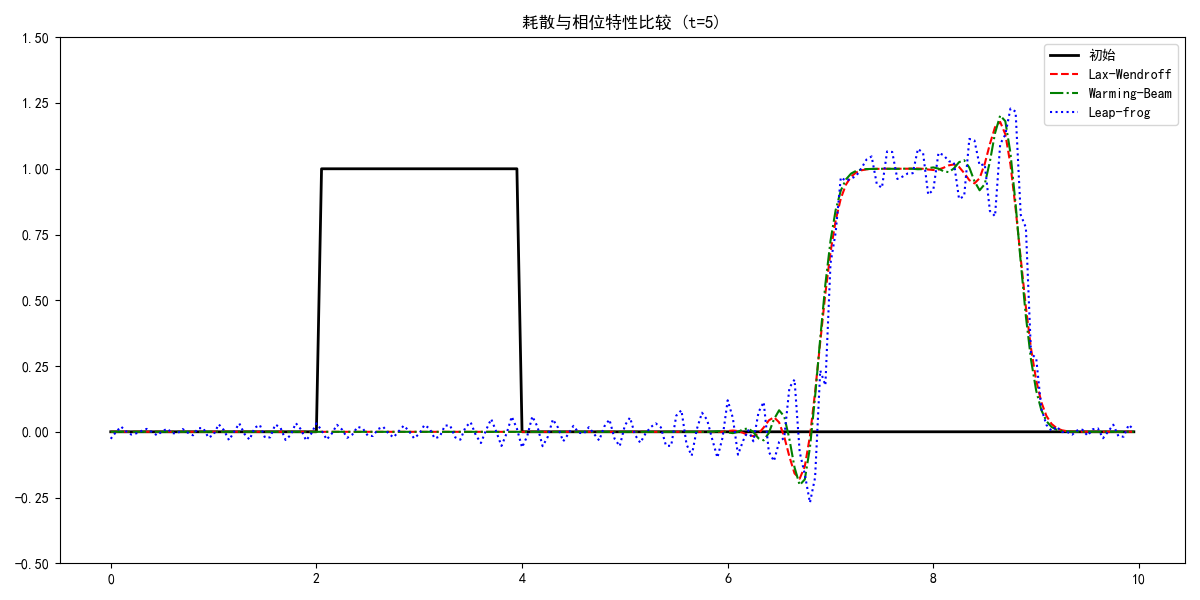
\includegraphics[width=0.9\textwidth]{Figure_3.png}
\caption{耗散与相位特性对比(黑色实线为初始方波)}
\label{fig:dissipation}
\end{figure}

\subsection{综合对比}
\begin{table}[htbp]
    \centering
    \caption{数值格式特性总结(基于图\ref{fig:stability}-\ref{fig:dissipation})}
    \begin{tabular}{l|ccc}
    特性         & L-W格式 & W-B格式 & Leap-frog \\ \hline
    CFL条件      & [0,1]   & [0,2]   & [0,1]     \\
    耗散性       & 弱      & 强      & 无        \\
    相位误差     & 滞后    & 超前    & 分裂      \\
    计算效率     & 高      & 最高     & 低        \\
    \end{tabular}
\end{table}

关键结论:
\begin{itemize}
    \item Lax-Wendroff适合光滑问题的高精度计算(见图\ref{fig:convergence})
    \item Warming-Beam可抑制高频振荡但牺牲精度(见图\ref{fig:dissipation}子图c)
    \item Leap-frog需严格控制$\sigma\leq1$避免振荡增长(见图\ref{fig:stability}子图f)
\end{itemize}
%附录
\newpage
\appendix
\section{AI工具使用声明表}
\begin{table}[H]
    \centering
    \begin{tabular}{c|c|c}
        \hline
        使用内容 & 工具名称 & 使用目的 \\ \hline
        hw3.tex 1-9行、图片插入 & Github Copilot & 调整pdf格式,调用宏包,省略插入图片的重复性工作 \\ 
        .gitignore & Github Copilot & 针对于python和latex的.gitignore文件,完全由Copilot生成  \\
        main.py 部分matplotlib部分 & Github Copilot & 省略图片绘制的重复性工作
    \end{tabular}
    \label{tab:AI_tools}
\end{table}
\end{document}